% Primero se crea un dataframe centralizado
% Se ponen los junctions en carpetas Desktop/Codes/Tesis/NNTrain/Drive/Explore/junctions.ipynb ok
% Se etiquetan manualmente Documents/DriveDatasetStable/Train/junc_tag.py ok
%//train_dataset_junctions.csv o train_dataset.csv
% Se crea un dataframe final con los nuevos atributos Desktop/Codes/Tesis/NNTrain/Drive/Explore/unify_df.ipynb
% Se modifica la red de conducción
% Se entrena la red de conducción
% Copiar la implementación del fastdepth https://github.com/dwofk/fast-depth
% Se entrena la red de profundidad con un softmax 2D

\section{PREPARACIÓN DE DATOS}
	% Desktop/Codes/Tesis/DataExtraction/df_processing.ipynb
	Una vez recolectados los datos se debe empezar a procesarlos para agregar atributos de utilidad para los modelos y seleccionar la información que nos interesa, todas las etapas están implementadas en el lenguaje Python.
	
	\subsection{UNIÓN DE DATAFRAMES}
		Se debe unir los dataframes en formato CSV en un solo archivo para poder realizar futuras etapas de pre procesamiento.
		
		\inputminted[frame=lines,
		baselinestretch=1,
		fontsize=\footnotesize,
		autogobble]{python}{codigos/marco-aplicativo/df_processing.py}
		\captionof{listing}{unión de dataframes}
		
		Se cargan los dataframes en una lista, la cual luego se itera para crear una nueva columna en cada uno, esta columna contiene el nombre de los archivos referenciados en el dataframe bajo la estructura \textit{carpeta/archivo}, para luego unirlos en archivo mediante la función \textit{concat} de la librería de manipulación de datos \textit{pandas}.
		
	\subsection{ETIQUETADO DE INTERSECCIONES}
		Luego de un estudio de los datos obtenidos, se decide etiquetar las intersecciones agregando nuevos atributos:
		
		\begin{itemize}[nosep]
			\item path left: indica si se tiene un camino a la izquierda disponible.
			\item path right: indica si se tiene un camino a la derecha disponible. 
			\item path forward: indica si se tiene un camino recto disponible.
			\item action left: indica si el vehículo tomó el camino por izquierda.
			\item action right: indica si el vehículo tomó el camino por derecha.
			\item action forward: indica si el vehículo tomó el camino directo.
		\end{itemize}
	
		Para mantener la consistencia, a las imágenes que no pertenecen a ninguna intersección se les asignó la etiqueta \textit{no action} especificando que no se toma acción alguna.
		
		Debido a las características del mapa, que todas las intersecciones son de tipo T, se debe tener la información de qué caminos se tiene disponibles a tomar, con el fin de ingresar este dato en la etapa de inferencia.
		
		\begin{figure}[H]
			\centering
			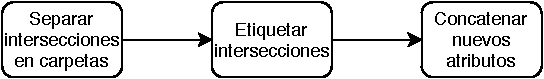
\includegraphics[scale=1]{imagenes/arquitectura_juncs}
			\caption[Etapas del etiquetado de intersecciones]{etapas del etiquetado de intersecciones}
			\label{junctions}
		\end{figure}
		
		Este etiquetado se debe realizar de manera manual, por lo que primero se detectan los fotogramas que componen las intersecciones, para esto se extraen todas las imágenes marcadas como intersección, se procede a calcular la diferencia de índices entre imágenes, si la diferencia es mayor a 1 entonces inicia una nueva intersección, repitiendo este procedimiento se finaliza la etapa de separación en carpetas (figura \ref{junctions}), los archivos de cada carpeta tienen como nombre el id de simulación de origen, y el nombre de archivo original, para al unificar la información de nuevo sea fácil saber de dónde proviene cada intersección.
		
		Inmediatamente se implementa un script que lea carpeta por carpeta y muestre los fotogramas que componen cada intersección como vídeo, para que así el etiquetador pueda ingresar los atributos codificados para el tipo de intersección y la acción tomada, codificado con los controles de dirección estándar en un teclado (wasd).
		
		\inputminted[frame=lines,
		baselinestretch=1,
		fontsize=\footnotesize,
		autogobble]{python}{codigos/marco-aplicativo/junc_tag.py}
		\captionof{listing}{interfaz de etiquetado}
		
	\subsection{CONCATENACIÓN DE ATRIBUTOS}
		En la etapa final del pre procesamiento, se deben concatenar las nuevas columnas de atributos al CSV del conjunto de datos, llenando con valores positivos para la etiqueta \textit{no action} en caso de no pertenecer a una intersección, para esta tarea se implementa un script que cree una lista de valores para cada entrada con valor por defecto 1 y se van asignando ceros para cada elemento de las intersecciones en base a los nombres de los archivos en cada carpeta.
		
		Así finaliza la etapa de pre procesamiento de datos con un CSV indexando todas las imágenes recolectadas con sus correspondientes etiquetas de aceleración, dirección y caminos en intersecciones.